% !TeX root = ../thuthesis-example.tex


\chapter{时间序列数据分析与处理}\label{chapter3}


\section{引言}
  在本章节中,对实验的情况进行了具体的说明,
  交待了实验环境,实验参数等。

  同时对数据相关的问题进行了阐述。
  对实验中用到的数据进行了说明,
  同时说明了数据预处理的流程和具体的方法,
  以及采用相关方法的动机、实际效果等。


\section{数据及评价指标说明}
  本文中应用的数据主要包括电网数据和列车走行部数据,都是实时采集的实际场景中的工业装备状态数据。
  下面对这两种数据的具体情况分别进行了说明。

  % !!!说明数据分别应用到了哪些地方
  \subsubsection{电网数据说明}
    本文实验中采用的电网数据,是基于青岛永磁实验台,
    按线路条件(包括牵引、匀速、制动),跑典型工况,采集的相关数据。

    数据在150t、192t、222t三种不同载荷下分别采集,
    在为10Hz、100Hz、100kHz三种不同采集频率的下,采集到不同特征列数据。

    在表\ref{tab:features2}中对各特征列进行了详细的说明。
    \begin{table}
        \centering
        \caption{电网温度预测模型中用到的主要特征说明}
        \begin{tabular}{lclclclcl}
          \toprule
          特征    & 通道名称 &采集频率&采集方式 &特征说明                                       \\
          \midrule
          电机温度   & AI\_Motor2Temp1\_gui &10Hz &PTU采集 & 待预测特征之一\\
          PU温度   & AI\_PUTemp\_gui &10Hz &PTU采集 & 待预测特征之一\\
          网流   & AI\_BusNegCurrent\_gui &10Hz &PTU采集 & 输入特征之一\\
          U相电流瞬时值   & AI\_PhaseUCurrent2\_gui &10Hz &PTU采集 & 输入特征之一\\
          U相电流有效值   & AI\_PhaseUCurrent2\_RMS\_gui &10Hz &PTU采集 & 输入特征之一\\
          W相电流瞬时值   & AI\_PhaseWCurrent2\_gui &10Hz &PTU采集 & 输入特征之一\\
          W相电流有效值   & AI\_PhaseWCurrent2\_RMS\_gui &10Hz &PTU采集 & 输入特征之一\\
          环境温度   & PT2\_ &100Hz &数采系统 & 输入特征之一\\
          电机速度   & Mot2\_speed\_rpm\_gui &10Hz &PTU采集 & 输入特征之一\\
          
          \bottomrule
        \end{tabular}
        \label{tab:features2}
      \end{table}
    !!!补充完整
  \subsubsection{列车走行部数据说明}
    本文实验采用的数据包含列车底盘(又名走行部)的监测数据,
    包含各轴承温度、驾驶档位、输出功率、环境温度、当前轨道的地理位置情况等相关数据。

    需要通过预测轴承温度的方式来判断轴承的运行状态。

    本文中实验用的是车号为5103的列车的数据,在表\ref{tab:features1}中对各特征列进行了详细的说明。
    在清洗完成后,还剩88401条可用数据,跨时234天,平均时间间隔为228.6秒,
    但是采样间隔分布比较不均匀,例如列车停运时采样间隔会比较长。

    \begin{table}
      \centering
      \caption{列车轴温预测模型中用到的主要特征说明}
      \begin{tabular}{ll}
        \toprule
        特征       & 特征说明                                       \\
        \midrule
        采集时间      & 用于数据分段和序列处理 \\
        车号          &\\
        1~6个轴的测试温度 & 待预测特征。共6个轴,每个轴六个测试点。 \\
        环境温度1、2  & 两个点采集到的环境温度,用于预测轴温的特征 \\
        主发电机温度  & 用于预测轴温的特征\\
        风机1、2温度  & 用于预测轴温的特征\\
        

        \bottomrule
      \end{tabular}
      \label{tab:features1}
    \end{table}
  \subsubsection{评价指标}
    均方误差(MSE,Mean squared error)是比较常用的反映估计量和被估计量之间差异程度的一种度量。
  
    但是均方误差作为评价指标也有它存在的问题。比较大的一个问题就是对异常值比较敏感,
    如果样本中有个别异常值出现,会对均方误差的影响比较大,导致评估的结果并不鲁棒。
  
    针对这个问题,在数据预处理的数据清洗阶段做出了一些处理,去掉了一些明显的异常点。
    % \subsection{数据集和实验基准说明}

\section{数据特点分析}
  \subsection{工业装备状态数据特点}
  工业装备数据一般采集于实际的工业装备系统,由于系统本身十分复杂,
  机理很难分析,很难对其进行建模分析。
  而且由于数据本身会存在噪声干扰,特性也比较复杂,
  通过传统的时间序列的分析方法也很难对其进行建模和抽取特征。
  
  \subsubsection{电网数据特点}
    \begin{enumerate}
      \item 电网数据来源于几种不同的采集方法,不同采集方法的采样频率会有差异。
      \item 如电压电流这类特征会有很明显的周期性。
    \end{enumerate}
  \subsubsection{列车轴温数据特点}
    \begin{enumerate}
      \item 数据波动十分剧烈。这份数据采集所在的区域所在的环境温度波动剧烈,
      如图\ref{fig:environment temperature change}所示,
      昼夜温差很大,低温低于15摄氏度,高温高于42摄氏度。
      
      \item 虽然在数据表中包含了地理位置信息,
      但是当前轨道的地理情况(坡度、弯度等)很难精确捕捉。
      \item 根据采集时间来看,列车的运行并不是一个连续的过程,
      会存在停运的情况,而且数据采集的过程也不连续。所以不能直接作为一个长时间序列来进行处理,
      需要对数据进行分段。
    \end{enumerate}
    \begin{figure}
      \centering
      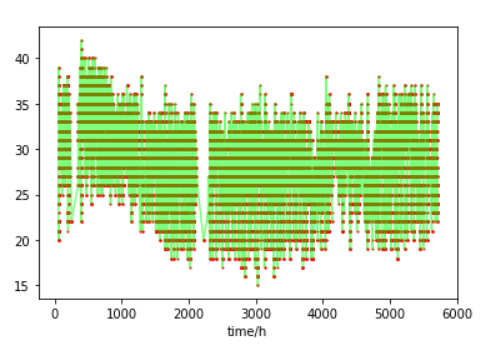
\includegraphics[width=0.8\linewidth]{figures/5303evn_tpt.png}
      \caption{5103号列车数据中环境温度变化图(横轴是时间,纵轴是环境温度,单位为摄氏度)}
      \label{fig:environment temperature change}
    \end{figure}

  \subsection{时间序列数据平稳性分析}
    \paragraph{平稳性分析的意义}~{}

    平稳性分析能够确定模型是否具有统计分析的意义。
    虽然利用深度学习建模并不是基于统计来对数据进行处理,
    但是平稳性分析能够检测序列是否具备被预测的基础,例如白噪声就不能被预测。

    这一个步骤主要是为了对待预测的数据的性质和预测难度有一个了解,方便后续选择合适的预测方法。
    
    % \paragraph{平稳性分析的具体方法和结论}~{} %Todo

\section{数据预处理}
数据的预处理包括如下的几个主要部分:数据读入、数据清洗、数据重采样、数据分段、数据标准化、
经验模态分解、数据窗口处理、划分训练集和测试集这些部分。下面会对这些内容分别进行阐述。
视数据特点的不同,个别的流程可能可以省略。
  \begin{figure}
    \centering
    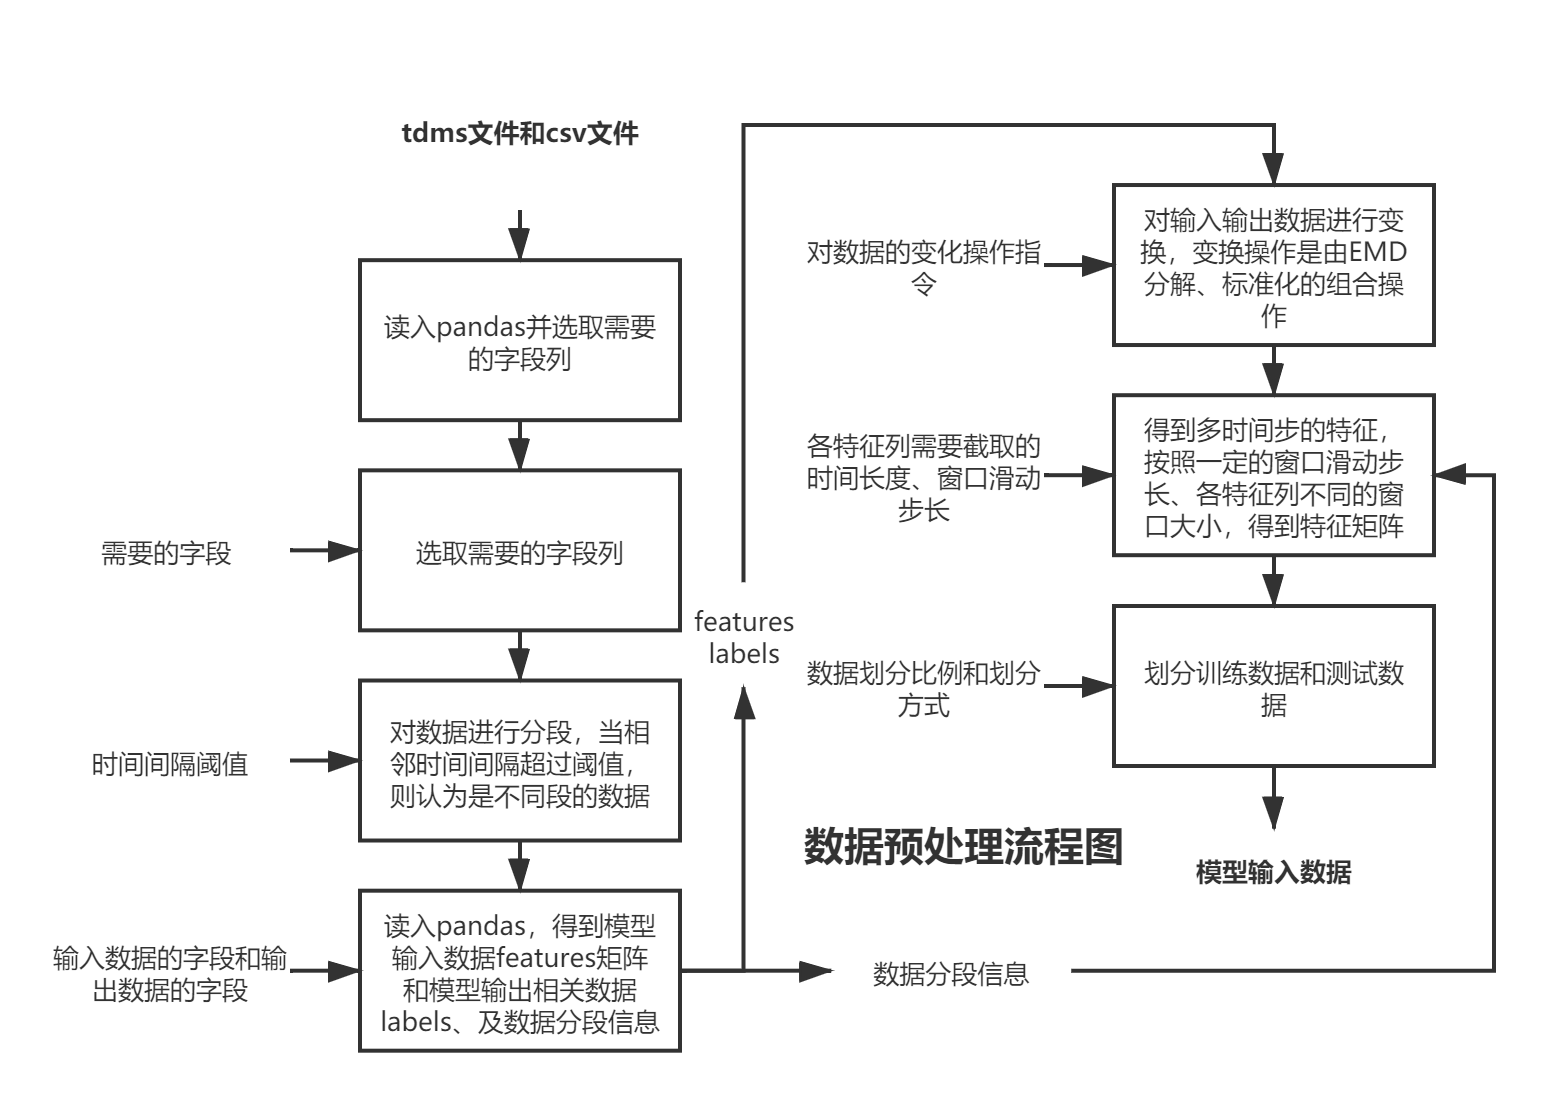
\includegraphics[width=1.1\linewidth]{figures/数据预处理流程.png}
    \caption{电网数据分段及划分处理流程图}
    \label{fig:data preprocess}
  \end{figure}
  \subsection{数据导入及清洗}
    电网原始数据存储在tdms文件和csv文件中,把数据读入pandas之后进行处理。
    列车轴温原始数据存储于dmp文件中,需要通过oracle数据库工具进行导入。

    在列车轴温数据中,导入后的数据存在问题。首先是存在着部分列的数据格式问题,
    打印出来发现是因为个别数据显示为“异常温度”或者是“-”。另外会有些数据的时间
    标记是默认的最小值的数据。
    用简单的处理数据缺失的方法来处理,由于数据量可观,可以直接在数据表
    中删除异常的样本点。

  \subsection{数据重采样}
  \begin{figure}
    \centering
    
    \begin{subfigure}[b]{0.45\textwidth}
        \centering
        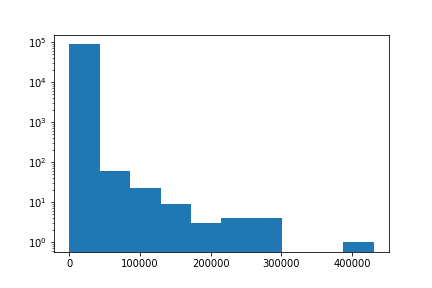
\includegraphics[width=\textwidth]{figures/time_intervals_distribution_log.png}
        \caption{采样间隔分布(log)}
        \label{fig:time_interval_log}
    \end{subfigure}
    \hfill
    \begin{subfigure}[b]{0.45\textwidth}
      \centering
      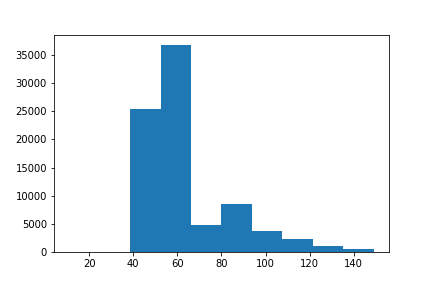
\includegraphics[width=\textwidth]{figures/time_intervals_distribution150.png}
      \caption{小于150秒的采样间隔分布}
      \label{fig:time_interval}
    \end{subfigure}
    
    \caption{列车走行部数据采样时间间隔分布直方图(横坐标:间隔(s),纵坐标:频次)}
    \label{fig:time intervals}
  \end{figure}
  需要注意的是,这一步对电网数据和列车轴温数据需要进行的操作是不一样的。
  
  在电网数据中,数据本身有固定的采样频率,采样间隔都是统一的,
  只是不同特征的采样频率不一样。

  但是在列车走行部数据中,如图\ref{fig:time intervals}中给出的采样时间间隔分布所示,
  采样点并不均匀的,就必须进行均匀间隔的重采样。

  \subsection{数据分段}
  首先介绍为什么需要对数据进行分段,在列车走行部数据中,如图\ref{fig:time intervals}中给出的采样时间间隔分布所示,
  采样点是十分不均匀的,间隔可能长达40000秒(约1天左右),也可能很短,50秒左右。
  如果只是进行简单的重采样,如果重采样的采样间隔过短,那在原始数据采样间隔很长的地方,
  会造成大量的数据冗余,对模型的训练也并没有好处;如果重采样的采样间隔过长,又会导致
  信息的过度丢失。

  所以这里提出一个数据分段的解决方案,通过设定一个合理的时间间隔阈值,如果两个点之间的
  时间间隔过长,我们则认为它们属于两个不同的数据段。

  关于时间间隔阈值的选择问题。可以将所有数据的时间间隔分布用直方图统计出来,
  再根据统计出来的结果选择出一条比较明显的分界线。

  为了找到重采样的合理阈值,这里对采样间隔进行了如\ref{fig:time intervals}直方图分析,
  大部分的采样间隔都集中在150秒以下,通过如\ref{fig:time_interval}
  中对150秒以下的间隔的进一步分析可以得到,70秒是一个比较合理的阈值。

  \subsection{整理数据表并通过滑动窗口取模型输入}
  在清洗完数据并对数据分好段之后,把需要用到的数据整理成一张二维的数据表。
  每一列是一个属性,每一行是一个采样点的数据。
  !!!滑动窗口示意图

  % \paragraph{输入输出的格式定义}~{} %Todo

  % 为了灵活方便,将输入输出定义为如下的字典格式:
  % \begin{minted}{Python}
  %     {(start_1, end_1) : [feature_1_1, feature_1_2, ...],
  %     (start_2, end_2) : [feature_2_1, feature_2_2, ...], ...}
  % \end{minted}

  % 其中start和end是相对时间而不是绝对时间。注意在input和output中相对时间的参考点需要一致。

  % 例如下面的定义方式,
  % \begin{minted}{Python}
  % input_attrs = {(-history_length, predicted_length) : features,
  %               (-history_length, 0) : labels} # 输入
  % output_attrs = {(0, predicted_length) : labels} # 输出
  % \end{minted}
  % 代表!!!


  \subsection{数据标准化}
  \begin{figure}
    \centering
    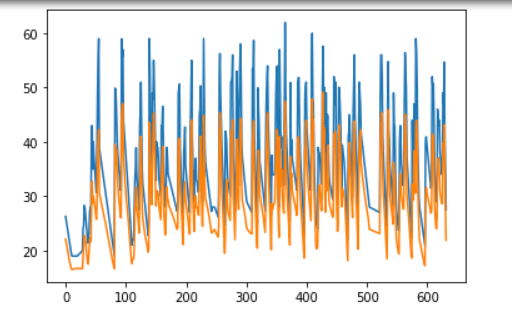
\includegraphics[width=0.8\textwidth]{figures/normalization.png}
    \caption{数据标准化前预测效果示意图}
    \label{fig:before normalization all points}
  \end{figure}
  数据预处理过程需要对数据进行标准化。如果没有标准化,会出现的问题是,
  预测趋势还是对的,但是对高温和低温的极值附近的预测很差,Accuracy结果比较好但是MSE差,
  这也是由于MSE的结果会比较受个别值的影响。
  如图\ref{fig:before normalization all points}所示。


  \begin{figure}
    \centering
    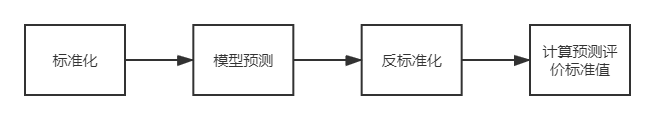
\includegraphics[width=\textwidth]{figures/标准化流程.png}
    \caption{数据标准化流程}
    \label{fig:pipeline of normalization}
  \end{figure}
  
  采用的标准化的方式是普遍被应用的控制均值和控制标准差的方式。
  具体的公式如\ref{eq:normalizaiton}所示,
  数据标准化的处理流程如\ref{fig:pipeline of normalization}所示,
  需要将预测结果反标准化之后再进行应用和计算评价标准的值。

  \begin{equation}\label{eq:normalizaiton}
    z=(x-u)/s
  \end{equation}

  其中,$u$是x的平均值,$s$是x的标准差。

  \begin{figure}
    \centering
    
    \begin{subfigure}[b]{0.45\textwidth}
        \centering
        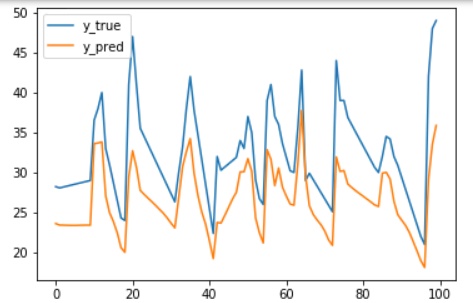
\includegraphics[width=\textwidth]{figures/normalization1.png}
        \caption{数据标准化前}
        \label{fig:before normalization}
    \end{subfigure}
    \hfill
    \begin{subfigure}[b]{0.45\textwidth}
      \centering
      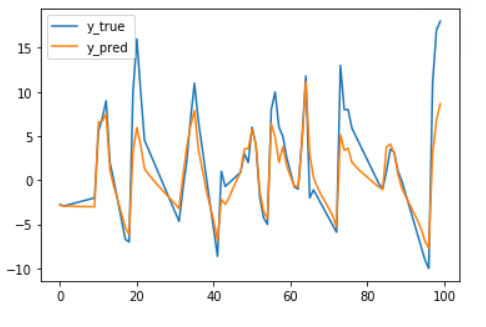
\includegraphics[width=\textwidth]{figures/normalization2.png}
      \caption{数据标准化后}
      \label{fig:after normalization}
    \end{subfigure}
    
    \caption{数据标准化效果说明图}
    \label{fig:normalization}
  \end{figure}

  为了更清晰的对比,在\ref{fig:normalization}中,截取了预测结果的片段进行对比。
  标准化前预测效果如\ref{fig:before normalization}所示。
  在加入标准化处理后,预测效果有了明显地改善。
  标准化后预测效果如\ref{fig:after normalization}所示。

  \subsection{不同序列划分方式}\label{subsection_diffrent_divide}
    训练集和测试集有如下两种不同的划分方式:
    \begin{enumerate}
      \item 第一种是序列化的顺序划分方式。
      以 7:3 的划分比例为例,即按照时间顺序,前 70\% 的数据作为训练集,后 30\% 的数据作为测试集。
      \item 第二钟是随机划分的方式。同样以 7:3 的划分比例为例,
      随机取70\%的样本点作为训练集,剩下30\%的样本点作为测试集。
    \end{enumerate}

    \begin{figure}
      \centering
      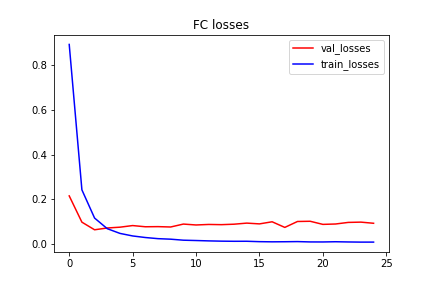
\includegraphics[width=0.5\textwidth]{20210327_1505/FC losses.png}
      \caption{出现过拟合问题的网络训练过程loss变化}
      \label{fig:overfit FC}
    \end{figure}
    
    \paragraph{序列化的划分方式下的过拟合问题}~{}

    不同的序列划分方式会导致实验结果有很大的差别。
    在序列化的划分时,很容易出现在训练集上效果很好,在测试集上效果不好的情况。
    图\ref{fig:overfit FC}是在序列化的样本划分方式下,
    应用全连接网络,训练得到的训练和验证集上的loss变化情况。
    如图\ref{fig:overfit FC},很明显训练出现了过拟合问题。
    分析原因是因为序列化的划分方式中的训练集和测试集,
    会由于工况的区别,有着很大的差异,给模型效果带来了挑战。

    但是在随机化的划分方式中则不容易出现这种问题。这也很容易理解,
    这和训练集和测试集的样本分布的相似度有关,随机划分的训练集和测试集的样本基本同分布。

    \paragraph{采样两种划分方式实验的原因}~{}

    这里之所以采用了两种划分方式进行实验,也是因为这两种划分方式各有其特点和不可替代的实际意义。
    序列化的划分方式更加接近实际中使用的场景,我们的模型在实际使用中,不可能将未来的数据拿来训练。
    但是由于资源的限制,实验用到的数据有限,而研究对象的情况会比较复杂,
    所以实际情况中会使用更多数据来训练模型,理论上当数据足够多时,会涵盖更多的数据情况,
    模型的应用效果也会更加接近随机划分训练集和测试集。

    实际的情况下模型的应用效果可能介于两种划分方式之间,所以这里对两种数据划分方式都展开了研究。
\section{实验环境}
    本文的实验都是在Linux系统下搭建完成,语言是Python,利用GPU进行模型的训练与测试。
  
    深度学习框架方面,本文的实验都基于Tensorflow 版本2.4.1进行,应用了Tensorflow2最新的Keras接口。
    具体的实验环境和安装包配置如表\ref{tab:env}
    \begin{table}
        \centering
        \caption{实验环境}
        \begin{tabular}{ll}
          \toprule
          环境        & 版本                                        \\
          \midrule
          操作系统        & Ubuntu 18.04.3 LTS                          \\
          Python      & 3.8                                         \\
          Tensorflow  & 2.4.1                                       \\
          Cuda        & V10.0.130      \\
  
          \bottomrule
        \end{tabular}
        \label{tab:env}
    \end{table}
    \subsection{实验说明}
    需要注意的是,为了消除随机因素的影响,
    如果没有特别说明,那文中给出的实验结果都是基于三次重复实验的平均结果。
    \subsection{选用Tensorflow2编写的原因}
    首先对比下动态图和静态图的特点。旧版本的Tensorflow一直采用的是静态图的机制,
    而被学术界研究人员广泛应用的Pytorch是基于动态图的机制。
    静态图是指,在图被构建之后,在模型运行之时,计算过程中,图是无法修改的。
    动态图反之,在计算过程中可以对图进行修改。
    由于静态图计算过程中图无法修改,所以可以在运行前进行一些优化例如融合部分Operation。
    但是也会因为图融合等原因,静态图在调试方面具有较大的难度,无法提供断点和单步调试功能,
    而且也会非常的不直观。
  
    Tensorflow不仅在部署上相对于其他框架有着独特的优势,而且Operation全面,生态良好。
    在升级Eager模式后,能够兼顾静态图运行效率快,和动态图代码简洁方便调试的优点。
  

\section{本章小结}


